\documentclass[12pt,a4paper]{article}
\setlength{\headheight}{16pt}
\usepackage[utf8]{inputenc}
\usepackage[spanish]{babel}
\usepackage{amsmath}
\usepackage{amsfonts}
\usepackage{amssymb}
\usepackage{graphicx}
\usepackage{fancyhdr}
\usepackage{float}
\usepackage{geometry}
\geometry{a4paper,left=2cm,right=2cm,top=2cm,bottom=2cm} 
%Para que no recorte las palabras con guiones
\tolerance=1000
\pretolerance=1000
% Símbolos de las unidades, sobre todo es para que en una ecuacion no queden en cursiva

\newcommand{\volt}{\mbox{V}}
\newcommand{\mvolt}{\mbox{mV}}
\newcommand{\hertz}{\mbox{Hz}}
\newcommand{\khertz}{\mbox{kHz}}
\newcommand{\Mhertz}{\mbox{MHz}}
\newcommand{\farad}{\mbox{F}}
\newcommand{\nfarad}{\mbox{nF}}
\newcommand{\pfarad}{\mbox{pF}}
\newcommand{\ohm}{\Omega}
\newcommand{\kohm}{\mbox{k}\Omega}
\newcommand{\Mohm}{\mbox{M}\Omega}
\newcommand{\amper}{\mbox{A}}
\newcommand{\mamper}{\mbox{mA}}
\newcommand{\segundo}{\mbox{s}}
\newcommand{\msec}{\mbox{ms}}
\newcommand{\usec}{\mu\mbox{s}}
\newcommand{\nsec}{\mbox{ns}}
\newcommand{\kwatt}{\mbox{kW}}

\providecommand{\E}[1]{\ensuremath{\times 10^{#1}}}
%para que al ir escribiendo se pueda poner \E{potencia} y quede:" x 10^potencia "

%------------------------- Inicio del documento ---------------------------

\begin{document}

%
% Sin cabecera ni pie de página:
%
\thispagestyle{empty}

\begin{figure}[t]
    \centering
    
\includegraphics [scale=0.72]{img/logo_fiuba_alta.jpg}
\end{figure}

\vspace{5.5cm}

\begin{center}
    \Large{Departamento de Electrónica}\\
    \huge{66.10 Circuitos Electrónicos II}\\
    \vspace{.5cm}
    \large{Proyecto: Amplificador de Audio de Potencia Clase G}\\
    \vspace{1cm}
    \begin{tabular}{lc}
    \textbf{Chaure Fernando} & 90389 \\
    \textbf{Combier Natasha} & Intercambio \\    
    \textbf{Marchi Pablo} & 90603 \\
    \textbf{Zurita Francisco} & 89722 \\ 
    \end{tabular}\\
    \vspace{.3cm}
    \small{\today}\\
\end{center}

\vspace{1.5cm}

\begin{center}
\begin{tabular}{|c|c|c|c|}
\hline
Cuatrimestre / Año & 1\sptext{er} cuatrimestre 2012 \\
\hline
Profesores: & Ing. Alberto Bertuccio \\

\hline
\end{tabular}


\vspace{1cm}
\begin{tabular}{|c|c|}
\hline
Fecha de entrega & Firma  \\
\hline
\hspace*{1cm} & \hspace*{3cm}\\
\hline

\hline
\end{tabular}

\vspace{.5cm}

\begin{tabular}{|c|c|c|c|c|}
\hline
\,Nota\, &\multicolumn{3}{|c|}{Fecha de aprobación} & Firma  \\
\hline
\hspace*{1.7cm} & \hspace*{1cm}& \hspace*{1cm} & \hspace*{1cm}  & \hspace*{3cm}\\
\hline
\end{tabular}

\vspace{1cm}
Obsevaciones:
\hrulefill\par
\vspace{.3cm}
\hrulefill\par
\vspace{.3cm}
\hrulefill\par
\vspace{.3cm}
\hrulefill\par
\vspace{.3cm}
\hrulefill\par
\vspace{.3cm}


\end{center}


\newpage
\thispagestyle{empty}
\tableofcontents
\newpage


%estilo de pie y encabezado de pagina
\pagestyle{fancy}
\lhead{66.10 Circuitos Electrónicos 2}
\fancyfoot[C]{1\sptext{er} cuatrimestre 2012}
\setcounter{page}{1}
\fancyfoot[R]{\thepage}


%Seciones y subseciones del tp

\section{Introducción}
\section{Introducción}
\bigskip

El presente informe detalla el diseño e implementación de un amplificador de audio clase G. En la realización de este proyecto han sido volcados los conocimientos de la materia Circuitos Electrónicos II. En la Figura~\ref{esquema_bloques}, se muestra el diagrama en bloques de las partes fundamentaes del proyecto.
	
	\begin{figure}[H]
	\centering
	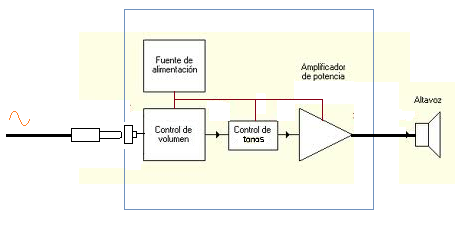
\includegraphics[scale=0.65]{img/esquema_bloques.png}
	\caption{Esquema en bloques.}
	\label{esquema_bloques} 
	\end{figure}
	
	
Un preamplificador es un circuito que permite adaptar las diferentes señales de entrada para luego poder ingresarlas a una etapa de potencia. Este circuito puede servir para adaptar señales de diferentes fuentes, por ejemplo: micrófonos, reproductores de mp3, salidas de placas de sonido de  pc, etc. Como todos estos dispositivos no tienen el mismo nivel de salida, el preamplificador es quien se encarga de llevar a todas estas señales a una tensión de estipulada que luego entra a la etapa de potencia anteriormente nombrada. Los preamplificadores suelen ser de baja potencia y de realizarse de forma adecuada no deben distorsionar en gran medida la señal.

Alguno de los controles que pueden tener los preamplificadores son:
	
\begin{itemize}
	\item Control de volumen
	\item Control de tono
	\item Control de balance
	\item Selector de canal de entrada 
	\item Amplificación
	\end{itemize}	
	
	
\subsection{Amplificadores de potencia}
	
Un amplificador debe satisfacer ciertos requerimientos especiales. Uno de los más importantes es el de entregar una señal con una cantidad específica de potencia a una carga con niveles aceptablemente bajos de distorsión. Otro objetivo común en el diseño es minimizar la impedancia de salida, de tal forma que la ganancia de voltaje quede relativamente poco afectada por el valor de la impedancia de carga. Una etapa de salida bien diseñada debe cumplir con estas características de funcionamiento, consumiendo poca potencia en estado de reposo, sin que esto represente una limitación importante en la respuesta en frecuencia del amplificador. 
 
Los amplificadores de potencia  se clasifican generalmente en seis tipos: A, B, AB , C y G para diseños analógicos y clases D y E para los diseños de conmutación. 
\medskip 


\subsubsection{Amplificadores clase A}


En esta clase de amplificadores se usa un solo transistor. El emisor seguidor es la etapa de salida clase A mas utilizada. La corriente de salida circula durante todo el ciclo de la señal de entrada, ya que el transistor esta polarizado con una corriente continua. Esta es una de las grandes desventajas de este tipo de amplificador ya que consume potencia en ausencia de señal y por lo tanto es lógico esperar un rendimiento pobre que en general no supera el 25\%. Como ventaja la distorsión introducida suele ser baja. En la Figura~\ref{ampliA} se muestra un ejemplo de este tipo de amplificador.
 
\begin{figure}[H]
\centering
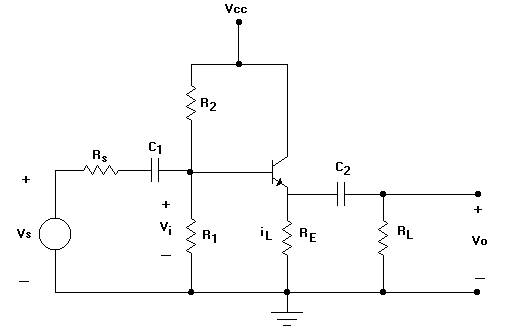
\includegraphics[scale=0.6]{img/ampliA.png}
\caption{Ejemplo, amplificador clase A}
\label{ampliA} 
\end{figure}

\medskip 
\subsubsection{Amplificador clase B}

Esta clase de amplificadores se compone de un par de transistores (uno pnp y otro npn) conectados de forma tal que no se encuentren ambos en la zona de modo activo directo en el mismo instante de tiempo. Es decir, si suponemos tener una entrada senoidal, durante un semiciclo uno de los transistores se encuentra en la región activa, conduciendo corriente, mientras que el otro se encuentra en corte y durante el otro semiciclo viceversa.
 Una ventaja de esta amplificador sobre la clase A, es que los transistores no disipan potencia en ausencia de señal, lo cual mejora la vida util de los transistores y el rendimiento notablemente, alcanzando un máximo del 78\%.
 La desventaja en este tipo de amplificadores es la llamada “distorsión por cruce”. Es fácil detectar su procedencia al analizar la Figura~\ref{ampliB}.

\begin{figure}[H]
\centering
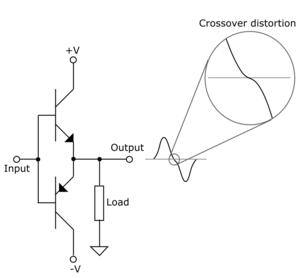
\includegraphics[scale=0.8]{img/ampliB.png}
\caption{Ejemplo, salida clase B.}
\label{ampliB} 
\end{figure}


Se observa que hay un intervalo de tensiones en el cual los transistores no conducen, ese rango generalmente esta dado por $\pm$0.7 V y esta dado por las curvas características de transferencia.

\medskip 
\subsubsection{Amplificador clase “AB”}


 Este tipo de amplificadores recurre a la misma topología utilizada en la etapa de salida de los amplificadores clase B, con la salvedad de que aquí en los transistores circulan una corriente de polarización a modo de reducir notablemente la “distorsión por cruce”.
 Existen diferentes formas de logra dicho tipo de polarización. Las mas sencillas implican agregar un resistor o diodos, por los que circula una corriente fija dada por el circuito de polarización o fuente de corriente. La otra forma es utilizar los circuitos conocidos como multiplicadores de VBE , que resulta ser la forma empleada en este trabajo práctico.

\medskip 
\subsubsection{Amplificador clase C}


La corriente de salida solo circula durante menos de medio ciclo de la señal de entrada. Y luego se complementa la salida con un circuito compuesto de capacitores e inductores.
La clase C trabaja para una banda de frecuencias estrecha y resulta muy apropiado en equipos de radiofrecuencia. Esto es debido al fenómeno de resonancia el cual se genera a la salida del amplificador cuando es sintonizado (la impedancia capacitiva e inductiva se cancelan a una frecuencia previamente calculada), aunque no trabaja arriba de 180 grados de ciclo, este amplificador a la salida genera una señal de ciclo completo de señal para la frecuencia fundamental. En la Figura~\ref{ampliC} se muestra un ejemplo de una amplificador de esta clase.
No se utiliza en sonido, por su gran nivel de distorsión y por que su operación no esta destinada para amplificadores de gran señal o gran potencia.

\begin{figure}[H]
\centering
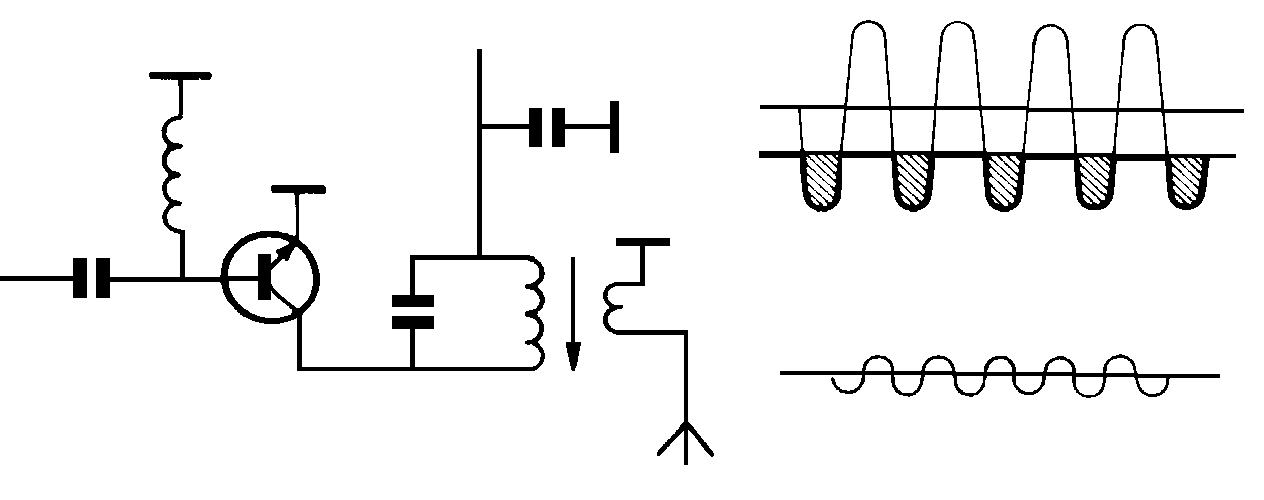
\includegraphics[scale=0.35]{img/ampliC.png}
\caption{Ejemplo, amplificador clase C.}
\label{ampliC} 
\end{figure}

\medskip 
\subsubsection{Amplificador clase D}

Esta clase de amplificadores usa señales de pulso (digitales). El uso de técnicas digitales hace posible obtener una señal que varía a lo largo del ciclo completo para producir la salida a partir de muchas partes de la señal de entrada. La principal ventaja de la operación en clase D es que los transistores MOSFET de salida trabajan solo en corte y saturación por lo que teóricamente no se disipa potencia en forma de calor y la eficiencia general puede ser muy alta, de entre 90\% a 99\%. En la practica los MOSFETS solo disipan potencia cuando se encuentran conduciendo (saturación) debido a la pequeña resistencia de encendido que poseen, llamada $R_dson$, de todas maneras esta potencia es despreciable ya que $R_dson$ es del orden de las milésimas de ohm. Se utilizan transistores MOSFET ya que son los únicos capaces de conmutar a las elevadas frecuencias de trabajo, del orden de las centenas de KHz llegando a los MHz en algunos casos.

\medskip 
\subsubsection{Amplificadores clase G}


Un amplificador clase G funciona conmutando fuentes de alimentación. Para analizar su funcionamiento tendremos en cuenta un circuito básico como se muestra en la Figura~\ref{ampliG}. Mientras el nivel de la señal de entrada sea pequeño (dentro del margen de +/- V1), el amplificador toma la potencia de la fuente V1. Si la señal de entrada excede el nivel de tensión dado por V1, el circuito automáticamente corta el suministro dado por V1 y conmuta a la fuente de alimentación V2 como puede verse en la Figura~\ref{ampliG_salida}. De esta forma la disipación de potencia es compartida por los transistores de salida, logrando así una menor disipación de potencia y una mayor eficiencia.
En la práctica, la clase G se considera linealmente pobre, comparada con la clase B, dado que la conmutación de las fuentes de alimentación se realiza mediante unos diodos, dando de esta manera un resultado alineal, ya que los mismos deben almacenar y desalojar cargas.
 
\begin{figure}[H]
 \centering
 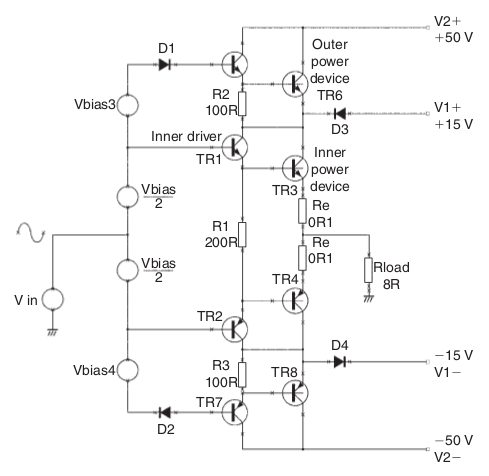
\includegraphics[scale=0.55]{img/ampliG.png}
 \caption{Ejemplo, amplificador clase G.}
 \label{ampliG} 
 \end{figure}
  
\begin{figure}[H]
 \centering
 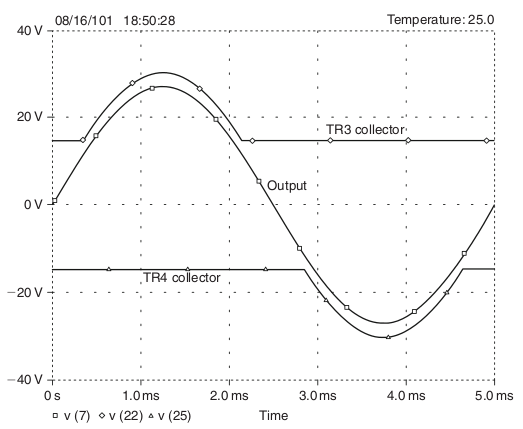
\includegraphics[scale=0.55]{img/ampliG_salida.png}
 \caption{Encendido de fuentes V2 en salidas clase G.}
 \label{ampliG_salida} 
 \end{figure}

\subsection{Principales especificaciones de un amplificador}
\medskip 
\subsubsection{Potencia máxima}

Potencia máxima eficaz, o potencia media a régimen continuo es la potencia eléctrica real verificable con instrumentos que puede proporcionar la etapa de salida  a una frecuencia de 1 kHz (frecuencias medias) sobre la impedancia nominal especificada por el fabricante (normalmente 4$\ohm$, 6$\ohm$ u $8\ohm$) y viene dada por la expresión $P_O=  \frac{V_{O(rms)}^2}{Z_O}$. Donde:
\begin{description}
\item $P_O$ es la potencia de salida
\item $V_{O(rms)}$ es la tensión eficaz de salida
\item $Z_O$ es la impedancia de salida
\end{description}

Se especifica la potencia máxima del amplificador en función de una determinada impedancia, generalmente $8\ohm$. Por ejemplo: 100 WRMS sobre 8$\ohm$.
Cabe destacar que si el amplificador es estéreo hay que tener en cuenta si la potencia se refiere a      ambos o a cada uno de los canales.
\medskip 
\subsubsection{Respuesta en frecuencia}

Es un rango de frecuencias dentro del cual el amplificador responde de igual forma (respuesta plana). Este rango se espera que como mínimo incluya las audiofrecuencias ( 20 a 20.000Hz)
Pueden especificarse las frecuencias de corte, en donde la potencia cae a la mitad o la tensión de salida cae en 3db o sino un rango de frecuencias en donde se cumple que la variación en la tensión de salida no supera una cota dado por el fabricante.
\medskip 
\subsubsection{Rango dinámico}

El rango dinámico(DR) es el conjunto de valores entre los niveles de mayor y menor salida, en donde el amplificador reproduce fielmente. En general viene especificado en decibeles y en donde el límite superior esta acotado por la distorsión mientras que el menor esta restringido por el ruido de salida. El rango dinámico se calcula con la relación entre ambos limites, de la siguiente forma:

\begin{equation}\label{rango_dinamico_eq}
DR= \frac{S+N}{N}
\end{equation}

donde:
\begin{description}
\item S es la señal máxima permitida
\item N es la señal de ruido
\item DR es el rango dinámico
\end{description}
\medskip 
\subsubsection{Distorsión armónica total}

Si en un sistema no lineal introducimos un tono de frecuencia $f_0$, en la salida tendremos ese mismo tono (con una amplitud y fase posiblemente diferentes) y, sumado a el, otros tonos de frecuencia $2f_0, 3f_0, ...$ llamados armónicos del tono fundamental . Por lo tanto la THD se calcula de la siguiente forma:

\begin{equation}\label{THD_eq}
THD= \frac{\sum Potencia~de ~los ~armonicos}{Potencia~ de ~la ~frecuencia fundamental}=\frac{P_0+P_1+...+P_N}{P_0}
\end{equation}

Es decir, la distorsión armónica es el valor rms de componentes armónicos de la señal de salida, expresadas como un porcentaje rms del fundamental.
Visto de otra forma, la distorsión describe la variación de la forma de onda de la salida del equipo, con respecto a la señal esperada, si el sistema fuese lineal, con respecto a una determinada entrada y se debe básicamente a la alinealidad de los mismos.
\medskip 
\subsubsection{Distorsión por intermodulación}


Es la distorsión que se produce cuando dos o mas señales atraviesan simultáneamente un sistema no lineal. Si dos tonos son reproducidos a la vez, pueden interactuar entre sí en el equipo y producir, asimismo, otros nuevos tonos, que son ni más ni menos que la suma y la diferencia de los dos tonos originales (es lo que se conoce como la frecuencia de batido o pulsaciones). Generalmente, los nuevos tonos no son armónicos entre sí ni con los anteriores debido a que la señal salida no es una combinación lineal de la entrada.
\medskip 
\subsubsection{Distorsión por intermodulación transitoria}


Este tipo de distorsión se da principalmente por el retardo que sufre la señal al ser realimentada negativamente. Todo amplificador demora un tiempo entre que la señal de entrada es aplicada y se obtiene la salida correspodiente, llamado tiempo de tránsito. Es decir, cuando utilizamos una realimentación negativa es esperable que al colocar una entrada inmediatamente obtengamos un efecto de la realimentación que afecte a la misma, pero debido a este tiempo de tránsito aparece un efecto no deseado y por lo tanto este tipo de distorsión. Esta altamente relacionada con el slew rate y con el ancho de banda a lazo abierto del sistema. 
\medskip 
\subsubsection{Slew rate}
	
Es la máxima pendiente que puede tener la tensión de entrada sin sufrir deformaciones se mide generalmente en $\frac{V}{\usec}$ y se calcula como:
\begin{equation}
SR = F(max) \times 2\pi \times V_p
\end{equation}
\begin{description}
\item F(max)= Frecuencia máxima de operación
\item  $V_p$= Tensión pico de onda
\end{description}
\medskip 
\subsubsection{Sensibilidad}

Este parámetro es una relación entre el valor de tensión de entrada que es necesario para producir la máxima potencia de salida y dicha señal de salida.Por lo general se especifica en decibeles a una determinada impedancia. Si la señal de entrada supera el valor especificado por la sensibilidad no existe ninguna garantía que la señal de salida no sufra un recorte que termine dañando algún componente.
\medskip 
\subsubsection{Relación señal a ruido}

La relación señal/ruido se define como el cociente que existe entre la potencia de la señal que se transmite y la potencia del ruido que la corrompe. Este margen es medido en decibeles. A su vez también es importante definir la figura de ruido. La magnitud del ruido generado por un dispositivo electrónico, por ejemplo un amplificador, se puede expresar mediante la denominada figura de ruido (F), que es el resultado de dividir la relación señal/ruido en la entrada (S/R)ent por la relación señal/ruido en la salida (S/R)sal, cuando los valores de señal y ruido se expresan en números simples :

\begin{equation}
F=\frac{(S/R)_{salida}}{(S/R)_{entrada}}
\end{equation}
\medskip 
\subsubsection{Impedancia de entrada}


 Es la impedancia equivalente que vería un generador aplicado a la entrada del amplificador. Para el caso particular de este tipo de amplificador (de tensión) buscamos que sea relativamente alta y no carge a la etapa anterior. Claramente depende de la frecuencia de operación pero un valor tipico para el rango de audiofrecuencias es de 10K $\ohm$.
\medskip 
\subsubsection{Impedancia de salida}


Es la impedancia equivalente que vería un generador aplicado a la salida del amplificador. En el caso particular del amplificador de audio buscamos que sea muy baja dado que las cargas son relativamente bajas y de lo contrario nos acortarían la amplitud de la señal de salida. Claramente depende de la frecuencia de operación pero un valor típico para el rango de audiofrecuencias es de décimas o centésimas de $\ohm$.
\medskip 
\subsubsection{Factor de amortiguamiento}

Indica la relación entre la impedancia nominal del parlante a conectar y la impedancia de salida del amplificador. Un factor de amortiguamiento alto permite mayor control del movimiento de los 
altavoces (evita oscilaciones) y por tanto reduce la distorsión, especialmente en graves. 

%El desarrollo del trabajo fue encarado como un caso real de la vida profesional, en el cual se nos han dado las especificaciones y basamos en ellas nuestro diseño, tratando de ser lo mas eficientes al menor costo posible y con los productos que se pudieron encontrar en el mercado.
%	
%Durante el desarrollo del trabajo hemos ido encontrando inconvenientes, ya sea errores humanos o diferencias entre las simulaciones y la implementación material. Se detallaron dichos problemas ya que consideramos que contribuyen al proceso de aprendizaje del diseño real.
\newpage
\section{Objetivos}
\bigskip
El proyecto consiste en el diseño e implementación de un amplificador de audio que cumpla con las siguientes especificaciones.

\medskip 
\paragraph{Especificaciones iniciales (típicas) de diseño:}

\begin{itemize}
\item Potencia de Salida: desde 25 W a 100 W RMS @ 8 $\ohm$

\item Salida Clase G

\item  Distorsión amónica total(THD): $<$ 0.002 \% a 1 kHz ,$<$ 0.01\% a 10 kHz: 20W (Baja tensión)
\item  Distorsión amónica total(THD): $<$0.003 \% a 1 kHz , $<$ 0.02\% a 10 kHz: 50W (Alta tensión)
\item Respuesta en frecuencia: +/-0.1 dB, 10 Hz – 30 kHz
\item SNR: $<$ -85 dB (20 Hz – 20 kHz)
\item Offset DC: $<$ +/-25 mV
\item Impedancia de entrada: 10 kohm
\item Sensibilidad: 1V RMS
\item Protección por cortocircuito y sobrecarga a la salida
\item Alimentación: 220 VAC +10/-20\%,50 Hz
    – Baja tensión: ~ +/-20V a +/-25V (Fuente lineal)
    – Alta tensión: ~ +/-35V a +/-50V (Fuente conmutada)
\item  Eficiencia:$>$70\%

\end{itemize}
\medskip 
\paragraph*{Características opcionales:}

\begin{itemize}
\item  Control de volumen VCA
\item  Boost +10 dB @ 30 Hz
\item  Ecualizador gráfico 5 bandas: $+/-$12 dB @64Hz, 250Hz, 1kHz, 4kHz, 12kHz
\item  Modulador / Demodulador FM para Public Adress

\end{itemize}
\newpage
\section{Desarrollo}

\subsection{Cálculos del Amplificador de Audio}
\subsection{Diseño del Amplificador de Audio}
\bigskip


\subsubsection{Primer Análisis}
 
El planteo comenzó focalizandose en un circuito mucho mas sencillo para el análisis. Por ende nos planteamos comprender el funcionamiento de un amplificador elemental con salida clase B como el de la Figura~\ref{idea_basica}.



\begin{figure}[H]
\centering
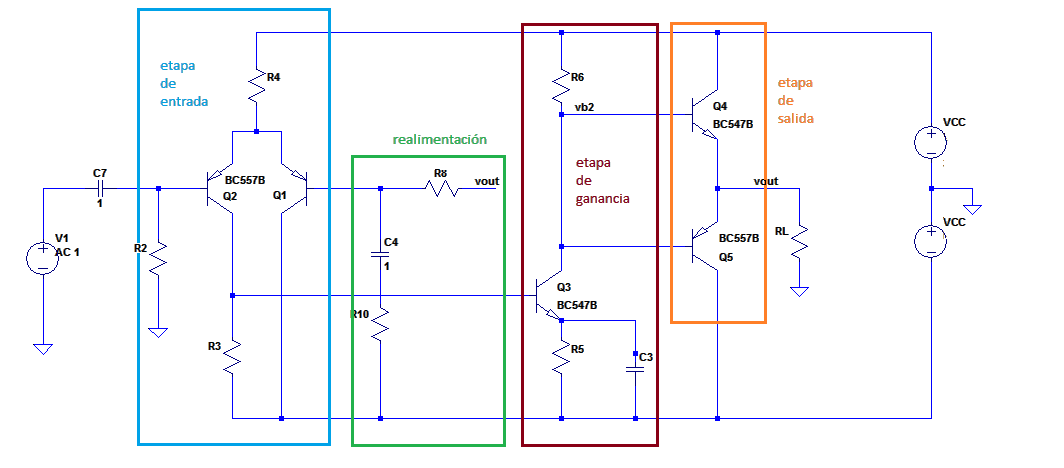
\includegraphics[width=0.8\textwidth]{img/idea_basica.png}
\caption{Amplificador simplificado.}
\label{idea_basica} 
\end{figure}

El primer desafío constó en plantear una correcta polarización. Al encontrarse el circuito realimentado negativamente es esperable que la tensión de continua en el nodo de salida $V_{out}$ sea muy cercana a cero. Este resultado puede comprenderse analizando el par diferencial y el efecto de la realimentación. Cuando el transistor Q2 se encuentre polarizado su tensión de base sea muy pequeña dado que circula una corriente baja. Por lo tanto, si la tensión $V_{out}$ no fuese un valor cercano a cero ya sea un valor negativo o positivo, produciría una tensión sobre el terminal de la base de Q1 distinto del correspondiente a Q2. Esto produciría que la corriente de Q2 se incremente o baje con respecto a la de Q1 y la salida también se vea afectada. Planteando que  $V_{out}$ aumentara:
$$
V_{out} \nearrow  ~ \Rightarrow V_{EB1} \searrow ~\Rightarrow I_{C1} \searrow ~\Rightarrow I_{C2} \nearrow ~\Rightarrow V_{B3} \nearrow ~\Rightarrow I_{C3} \nearrow \Rightarrow V_{B4} \searrow ~\Rightarrow V_{out} \searrow
$$

Siguiendo con este razonamiento si asumimos que $V_{out}$ es cercano a 0 volts. Entonces analizando el circuito llegamos a las siguientes ecuaciones:

\[
\frac{V_{CC}}{R6} = \frac{(V_{E3} - (-V_{cc})}{R5}
\]

$$
V_{E3} = V_B{3} - 0.7V
$$

Donde:
\begin{description}


\item $V_{B3} = (IC1 \times R_3 - V_{CC}) $
\item $I_{C1}=\frac{(V_{CC}-0.7V)}{2R_4}$
\item $V_{E3}= (V_{CC}-0.7) \frac{R3}{2R4} - V_{CC} - 0.7V$
\item $V_{CC} R5/R6 = \left[  (V_{CC}-0.7V) \times \frac{R_3}{2R_4} - 0.7V\right] $
\end{description}

Aproximando obtuvimos la siguiente relación:

$$ V_{CC} \times \frac{R_5}{R_6} + 0.7 =V_{CC} \times \frac{R_3}{2R_4} $$

Notando que el termino $\frac{R_5}{R_6}$ debía ser menor que la unidad debido a que $R_5$ es una resistencia de realimentación para la estabilidad de la polarización y $R_6$ es la que define la ganancia de esa etapa, y suele ser bastante alta para tener una alta ganancia de lazo abierto. 
Al tener una alta ganancia a lazo abierto la ganancia de lazo cerrado queda completamente definida por el realimentador. Observando el circuito:

$$ V_{out}= V_{in} \times \left(  1+\frac{R_8}{R_{10}} \right) ~ \Rightarrow ~ A_V= \left( 1+\frac{R_8}{R_{10}}\right) $$


Utilizando la sensibilidad requerida en las especificaciones,se estipula que al tener 1V rms en la entrada debemos tener máxima potencia de la señal de salida, asignamos a $R_8 = 22\kohm$ y a $R_{10} = 1\kohm$. De esta manera se obtiene una ganancia de 23 veces con una potencia máxima de 66 Wrms sobre una carga de $8 \ohm$ cumpliendo con los requisitos. Asignando una tensión de alimentación de $V_{cc}=35V$, simulamos el circuito:

\begin{center}
\parbox{0.5\textwidth}{
--- Operating Point ---
\begin{tabbing}
\hspace{3cm}\=\hspace{4cm}\=\hspace{5cm}\=\kill
I(Rl): \>	 -0.000492201 \>	 device$\_$current \\ 
Ie(Q1):	\> 0.000392712	\> device$\_$current \\ 
Ie(Q2):	\> 0.00116932	\> device$\_$current \\ 
I(R8):	\> -4.57521e-007\>	 device$\_$current \\ 
I(R6):	\> 0.000730688	\> device$\_$current \\ 
I(R5):	\> 0.000731219	\> device$\_$current \\ 
I(R3):	\> -0.00116632	\> device$\_$current \\ 
I(R2):	\> -1.36041e-006\>	 device$\_$current \\ 
I(R4):	\> 0.00156204	\> device$\_$current \\ 
\end{tabbing}
}
\end{center}

\begin{figure}[H]
\centering
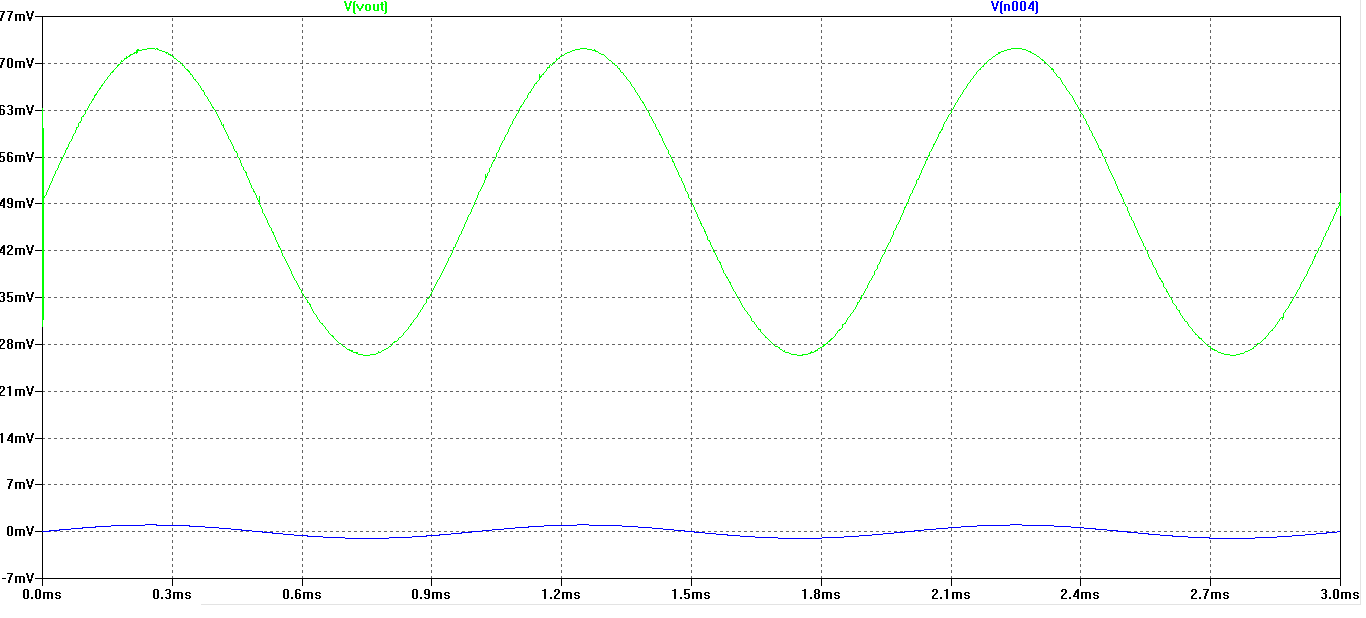
\includegraphics[width=\textwidth]{img/ganancia_1er_cir.png}
\caption{Respuesta temporal del $1^{er}$ prototipo.}
\end{figure}

\begin{figure}[H]
\centering
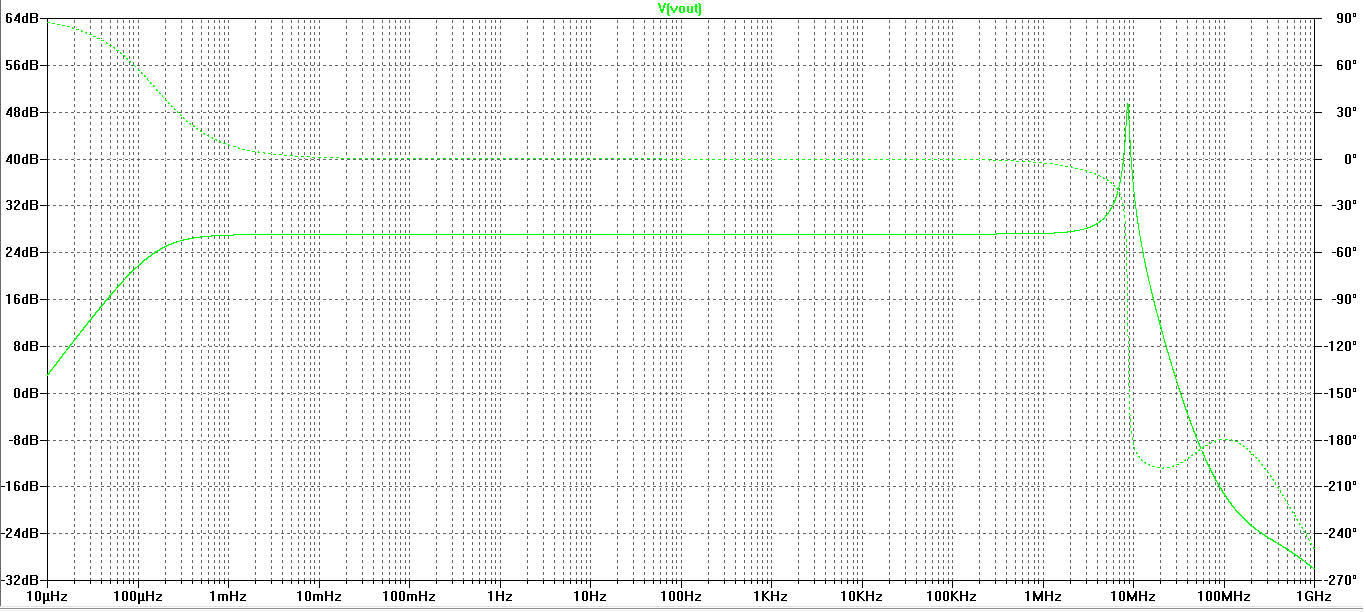
\includegraphics[width=\textwidth]{img/cir_basico_oscilante.png}
\caption{Respuesta en frecuencia del $1^{er}$ prototipo.}
\end{figure}

Los valores asignados fueron elegidos con el criterio de lograr una corriente de alrededor de 1mA para la etapa de entrada y de una relación entre $\frac{R5}{R6}$  de 0.001 veces. Obteniendo el resultado de que el circuito amplifica 22.85 veces y posee una alta inestabilidad.
Notar que el circuito simulado posee una resistencia de carga de 100 $\ohm$. Realizando una simulación habiendo compensado el circuito para que no se produzcan oscilaciones se obtuvo:

\begin{figure}[H]
\centering
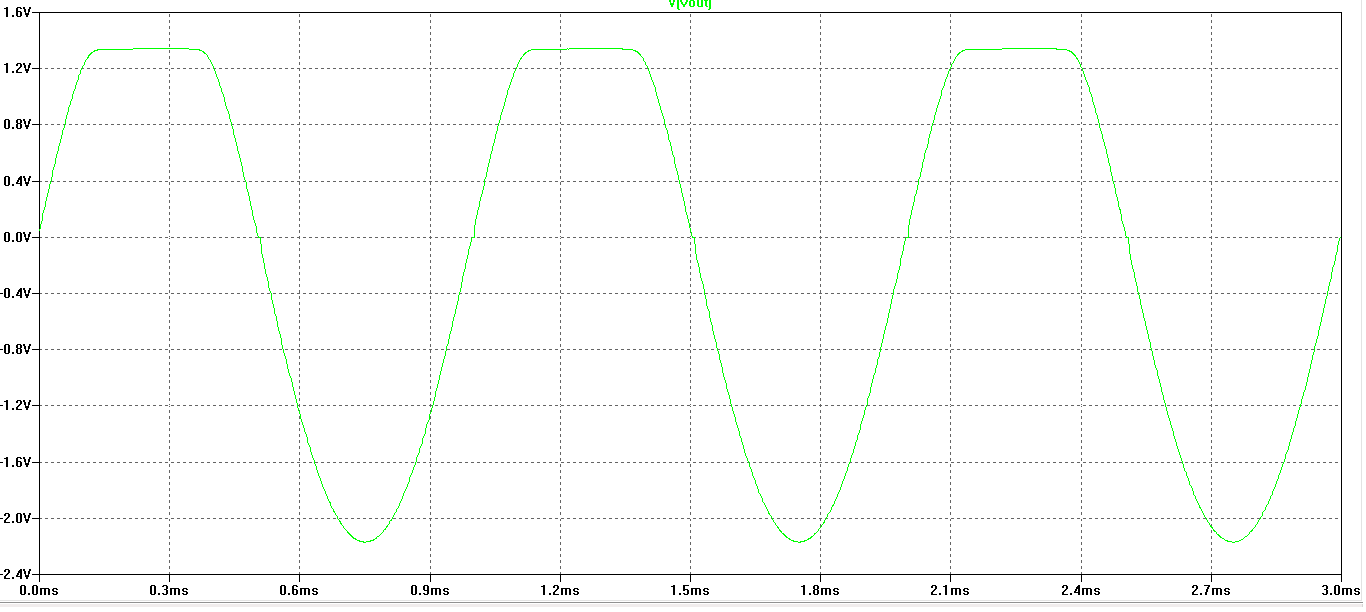
\includegraphics[width=\textwidth]{img/cir_basico_compensado.png}
\caption{Respuesta temporal luego de compensar.}
\end{figure}

Como puede observarse otro cambio que deberíamos lograr era bajar la resistencia de salida del circuito para que etapa de salida pudiese entregar mayor potencia sin llegar al recorte. Por ende aplicando una cantidad significativa de cambios pasamos a analizar el siguiente circuito:

\begin{figure}[H]
\centering
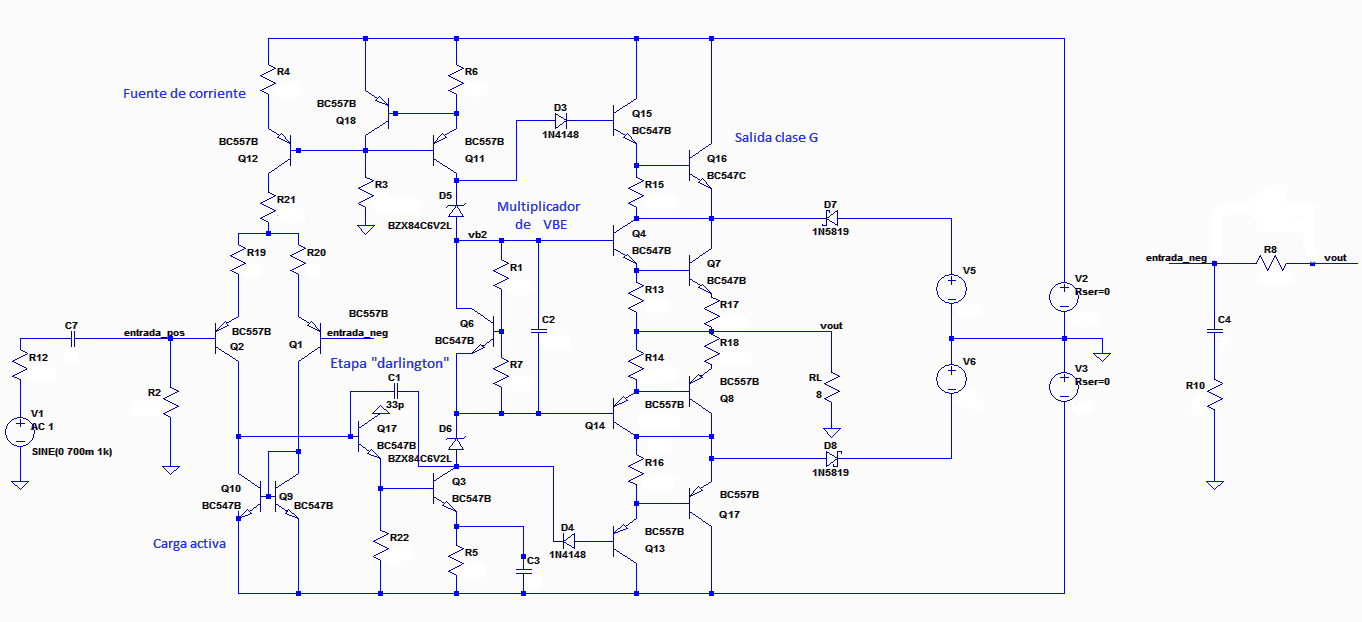
\includegraphics[width=\textwidth]{img/circuito_beta_mejorado.png}
\caption{Amplificador básico con algunas mejoras.}
\end{figure}

La primer diferencia que podemos apreciar es el reemplazo de la resistencia $R_4$ del circuito anterior por una fuente de corriente. Este cambio logra que la corriente de polarización del par diferencial sea mas estable frente a variaciones tanto por parte de la fuente de alimentación como así también por la temperatura de operación. Esta corriente es vital para definir las propiedades de pequeña señal y las distorsiones que puedan ocurrir en la primer etapa.Ademas aumenta su relación de rechazo en modo común.
Para calcular dicha corriente recorreremos la malla de control de dicha fuente aplicando la ley de Kirchhoff obtenemos que:
$$
V_{2} - V_{R4} - V_{BE Q12} + V_{BE Q11} + V_{R6} - V_{2} = 0
$$
Asumiendo que los dos transistores son exactamente iguales podemos asumir que sus $V_{BE}$ también lo serán. Por ende:
$$
- I_{C Q12} * R_{4} + I_{C Q11} * R_{6} = 0
$$
Llegando a la siguiente relación:
$$
I_{C Q12} = I_{C Q11} \times \frac{R_6}{R_4}
$$
\\
Por ende las corrientes $I_{C Q12}$ e $I_{C Q11}$  quedan determinadas por la relación entre $R_6$ y $R_4$. Para calcular la corriente $ I_{C Q11}$ realizamos la suposición de que el la tensión $V_{BE Q18}= 0,7V$ y en consecuencia $I_{C Q11}= {V_{BE Q18}}/{R_6}$. Los valores de resistencias normalizados adoptados logran que la corriente del par diferencial se mantenga alrededor de 1 mA. Este valor lo establecimos como norma, ya que valores mayores incorporarían más ruido a la primera etapa, y valores menores disminuirían la ganancia.

La segunda gran diferencia es la aplicación de una carga activa en reemplazo de resistores en el par diferencial lo cual nos introduce un aumento en la amplificación sumado a que se logra un lazo de realimentación que estabiliza la polarización, es decir, tiende a igualar las corrientes por ambas ramas del amplificador diferencial, disminuyendo los efectos de los desapareamientos e impidiendo la aparición de distorsión por $2^{da}$ armónica.

La tercer diferencia radica en la modificación de la etapa de ganancia por una etapa darlington para aumentar aun más la ganancia de lazo abierto. Además en esta etapa se ha colocado un capacitor, $C_1$, entre la base y el colector, de lo que sería $Q_3$ del circuito anterior, que produce un polo dominante para altas frecuencias. Este tipo de compensación se basa en el hecho de que la ganancia de la etapa es lo suficientemente grande como para que la capacitancia reflejada por efecto Miller también lo sea. La ventaja es que con capacidades pequeñas se logra estabilizar el sistema y estas suelen venir incluidas en el circuito integrado. La realimentacion local que linealiza la etapa se ve incrementada tal que a fines prácticos elimina la distorsion por alinealidad totalmente. La carga del colector del VAS, $Q_9$, forma una fuente de corriente.

La cuarta diferencia es la utilización de un circuito adicional entre las bases de $Q_5$ y $Q_4$. Posee dos funciones elementales: la primera es establecer una corriente de polarización en los transistores de salida que produce una notable disminución de la distorsión por cruce por cero. Para entender este efecto analizamos el primer circuito planteado, como observamos cuando un transistor de la etapa de salida clase B se encuentre el conducción el otro se encuentra en corte. Al disminuir la tensión de la salida del emisor común ($2^{da}$ etapa) a niveles cercanos al cero, ninguno de los transistores se encuentra en la región activa y en ese instante se produce una deformación de la señal como se observa en la Figura~\ref{falta_Vbe}. Claramente este tipo de distorsión será mas apreciable a señales de baja amplitud donde los efectos son mas apreciables. Para modificar este comportamiento se agregaría una "fuente" de tensión entre las bases de la etapa de salida clase B. Esta fuente polariza ambos transistores y produce por los mismos una corriente constante dependiendo exponencialmente de su valor. Esta "fuente" es reemplazada por el multiplicador donde como se ha analizado en clase, si el mismo es alimentado con una fuente de corriente constante vale afirmar que:

$$
V_{CE Q6} = (\frac{R_1}{R_7} + 1 ) \times V_{BE Q6}
$$

\begin{figure}[H]
\centering
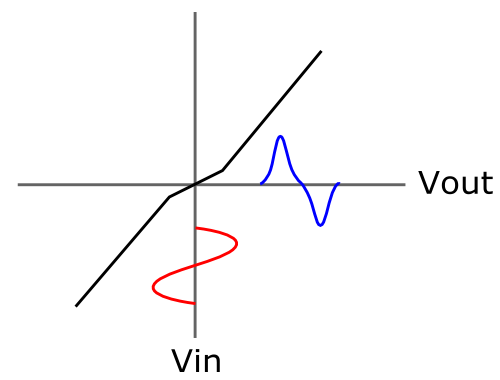
\includegraphics[width=0.5\textwidth]{img/falta_Vbe.png}
\caption{Deformación por falta de Multiplicador $V_be$}
\label{falta_Vbe}
\end{figure}

Ahora bien la segunda función elemental se observa en esta ecuación. El transistor $Q_6$ del multiplicador se acoplará termicamente con la etapa de salida de forma tal que si estos transisitores se embalan termicamente, es decir, un aumento de la temperatura produce un aumento de corriente que vuelve a producir un aumento de temperatura. Pero si el transistor $Q_6$ esta acoplado terminamente con la etapa de salida, al aumentar la temperatura pruducira una disminución en el valor de la tensión $V_{BE}$ (-2mV/$^o$C), disminuyendo la tensión $V_{CE Q6}$, bajando la corriente de los transistores y produciendo un lazo de realimentación negativa.

La quinta gran diferencia es la utilización de otro tipo de etapa de salida, la llamada clase G. Esto se relaciona al hecho de que quiere utilizarse para la reproducción de música, la cual, la mayor parte del tiempo se encuentra en niveles bajos y solo tiene picos temporales. Este hecho hace que sea eficiente el uso de una salida clase G.

En esta etapa los transistores están en configuración seguidor por emisor, ya que es sabida de ser menos propensa a oscilaciones parásitas o locales. $R_{15}$ y $R_{14}$  son los clásicos resistores de emisor para los drivers de bajas. Los drivers $Q_{12}$ y $Q_{15}$ tienen sus propios resistores de emisor $R_{13}$ y $R_{16}$, que cumplen su rol de establecer una razonable corriente en los drivers cuando se prenden a modo de incrementar su transconductancia y ademas acelerar el apagado de los dispositivos de altas al proveer una salida para los portadores de las bases de los mencionados dispositivos. Los colectores de los drivers están conectados a los rieles de altas para minimizar los saltos de ganancia causados por el cambio abrupto en la tension de colector cuando se produce la conmutación.

Cuando una tension positiva excede el riel de bajas, $D_3$ pasa a conducción,$Q_{15}$ y $Q_{16}$ se prenden mientras que $D_7$ se apaga y , por lo tanto, la corriente es suministrada  el riel de altas, con la caída de tension y consumo de potencia debidos a $Q_{15}$ y $Q_{16}$. Los picos de tensiones negativas tienen un desarrollo análogo.
La conmutación en la clase G trae acarreado un problema de alinealidad en los diodos de conmutación. Estos diodos en general deben conducir grandes cantidades de corriente antes de conmutar, y una consiguiente acumulación de cargas. Al conmutar las cargas acumuladan mantienen la corriente durante un corto tiempo mientras son barridas de la juntura. Esta corriente es suministrada por el transistor de altas. Cuando el diodo corta completamente, este exceso de corriente que conducía el transistor de altas pasa directamente hasta el de bajas y a la resistencia de degeneración. Este problema se puede eliminar con un diodo de alta recombinación, como ser el diodo Schottky de potencia, que son mas rápidos y acumulan menos carga.

Mientras la señal se mantenga en baja potencia, un amplificador de baja potencia lo hará mas eficiente. La mayor parte del tiempo son los rieles de baja tension los que proveen la potencia de salida, habiendo baja caída de tension entre riel y salida y consecuentemente, menor disipación. Pero, cuando aparecen picos de alta tension, se activan los rieles de alta tension, causando mayor gasto de energía durante esos cortos periodos de tiempo.



\bigskip

%La resistencia de entrada desacoplada por el capacitor C5 provee una resistencia de entrada de $10K\Omega$ para la señal y en continua se ven $22K\Omega$, equiparando con la realimentacion. De esta forma, se equilibra el offset producido por las corrientes de base del par diferencial, minimizando la tensión diferencial de offset.



%El principal inconveniente al compensar el circuito por polo dominantes es que al agregar un capacitor, este modifica el ancho de banda de potencia. Esto se debe al tiempo que le toma a la etapa anterior cargar el capacitor. Debido a esto la elección del valor de este capacitor debe tener en cuenta ambos efectos y buscar una relación de compromiso entre ambos.


%\subsubsection*{Slew Rate}
%
%El capacitor de compensación $C_1$ conectado alrededor del par Darlington hace que esta etapa actúe como un integrador, y la corriente que carga el punto de compensación es justamente $I_x$. 
%Se puede observar que la corriente máxima disponible para cargar C1 es 2$I_1$, donde $I_1$ es la corriente en reposo por cada dispositivo en la etapa de entrada. Es decir, a grandes valores de Vi las corrientes del par diferencial se desequilibran, $I_1$ crece hasta su valor máximo 2$I_1$ y la corriente por la otra rama del par se anula, por ende es fácil ver que por la carga activa deja de circular corriente y toda la corriente de la primer rama del par se transforma en $I_x$.
%El circuito por lo tanto opera en forma no lineal. Si la etapa de entrada actuara de forma lineal produciría una corriente $I_x$ muy grande y el slew rate no produciría ninguna limitación.
%
%\[
%	V_o= \dfrac{1}{C1} \int 2I_1\,\mathrm{d}t    
%\]
%
%$$
%	SR=\dfrac{dVo}{dt}=\dfrac{2I_1}{C1}
%$$
%
%Por lo tanto, realizando el calculo para nuestro circuito, siendo $I_1$ =2.2mA y C1=120pF. Obtenemos:
%$$ SR=36\dfrac{V}{\usec} $$


%$C_{13}$ y $R_{32}$ conforman la red Zobel encargada de hacer ver a la bobina como una carga resistiva. La red conformada por $L_{1}$ y $R_{33}$ aíslan al amplificador de carga capacitiva, aplanando la respuesta en frecuencia.


\bigskip
\subsubsection{Protección Contra Cortocircuitos}\label{contra_cortos} 

A modo de reducir las consecuencias de los accidentes, se agregaron además, circuitos de protección contra cortocircuitos. El funcionamiento básico es que usa los resistores de la salida para sensar la corriente que pasa por ellos. Cuando la corriente excede el valor máximo permitido, el cual se elige para una sobrecarga determinada (esto incluye el caso extremo de cortocircuito), la tensión que cae en esta resistencia enciende en transistor, el cual comienza a drenar corriente de la entrada de la etapa de salida, a fin de limitar la corriente de salida.
Un problema que se podría tener es el de tener un corto interno pero no notarlo, en cuyo caso las protecciones estarían constantemente en funcionamiento. Entonces, para notarlo, se reemplazo un diodo de las protecciones por un LED, a fin de que cuando las protecciones esten funcionando, el LED se polarice y su señal luminosa nos informe del problema.
\subsection{Cálculos de las Fuentes de Alimentación}
	\subsection{Diseño de las Fuentes de Alimentación}
\bigskip 

En líneas generales, todo el circuitos estará alimentado por cuatro rieles, dos de alta tensión y dos de baja. Los rieles de altas serán suministrados por una fuente lineal mientras que para los de bajas, se reducirá la tensión de los rieles altos con una fuente de switching.

\subsubsection{Fuente Lineal}

Para los rieles altos se opto por una fuente lineal. La misma consiste esencialmente de tres bloques:

\begin{itemize}
\item Transformador 220/36+36
\item Rectificador de onda completa
\item Divisor capacitivo 
\end{itemize}

El transformador reduce de 220$V_{rms}$ a 72$V_{rms}$, es decir, tensión pico de $72V_{rms}*\sqrt{2}=101.82V$.

Para el rectificador de onda completa se usaron diodos 6A10 en paralelo con capacitores de $100nF$ para reducir ruido. La caída en los diodos es de aproximadamente $0.7V$, reduciendo la tensión a la salida de este bloque a $101.82V-2*0.7V=100.4V$

Finalmente para el divisor capacitivo, se colocaron dos hileras de capacitores en paralelo, dando un divisor de $2200{\mu}F*4=8800{\mu}F$. El punto medio del divisor toma la tension de tierra, y los otros, $\pm50.2V$.


\begin{figure}[H]
\centering
\centerline{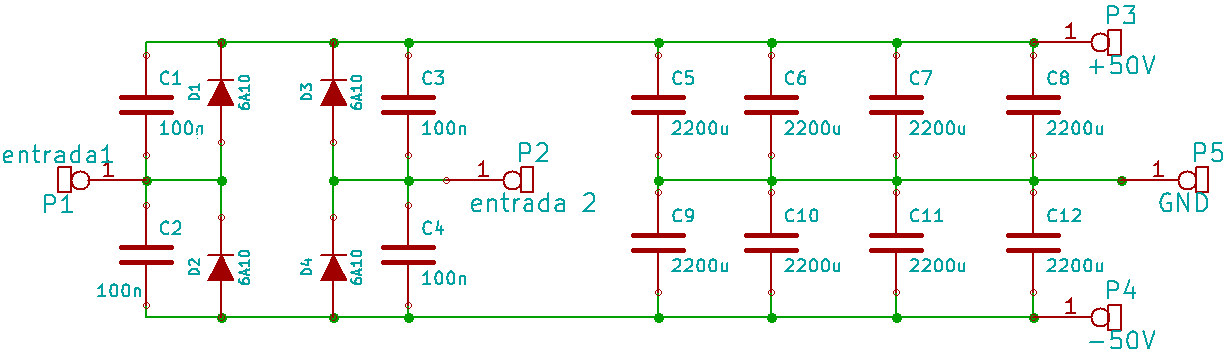
\includegraphics[scale=0.4]{img/esquema_fuente_lineal.png}}
\caption{Esquema de la fuente lineal}
\label{esquema_fuente_lineal} 
\end{figure}

\subsubsection*{Ripple}

Para calcular el factor de rizado $F_r=\frac{V_{ca}}{V_{cd}}$ vamos a separar los casos entre el riel alto y el bajo, porque no ven la misma carga.

El riel alto ademas de ver el amplificador, alimenta la fuente de switching, así que las impedancias de entrada quedan en paralelo, empeorando el factor de ripple. Aproximadamente la impedancia de entrada de la switching son $500\ohm$, despreciando todo menos la resistencia en serie que se ve del bobinado del relé y el bobinado del primario. Luego, $500\ohm$ en paralelo con la resistencia de entrada simulada del amplificador $1.8k\ohm$ es aproximadamente $400\ohm$.Ve también un capacitor de $220{\mu}F$.
Por tanto, el factor de rizado queda:

\[
	F_r=\frac{1}{\sqrt{3}(4fRC-1)}$$
$$	F_r=\frac{1}{\sqrt{3}(4\times 50Hz\times 400\ohm\times (8800+220){\mu}F-1)}$$
$$	F_r=0.00046
\]

El riel bajo ve aproximadamente $R_i=\frac{-50V}{-25mA}=2k\ohm$, valor de corriente obtenido por simulación sin señal. Ve también un capacitor de $220{\mu}F$.
Por tanto, el factor de rizado queda:

\[
	F_r=\frac{1}{\sqrt{3}(4fRC-1)}$$
$$	F_r=\frac{1}{\sqrt{3}(4\times 50Hz\times 2k\ohm\times (8800+220){\mu}F-1)}$$
$$	F_r=0.00016
\]

Para el peor caso de carga, es decir con una entrada de $V_i=1V_{rms}$, la carga vista será $R_i=\frac{-50V}{-4A}=12.5\ohm$ y $F_r=0.026$ en el pico del semiciclo negativo. Este caso será sumamente inusual de ver.


\subsection{Simulaciones}

\subsection{Realización del Circuito Impreso}
\subsection{Realización del Circuito Impreso}
\bigskip 
\subsubsection{Criterios de Diseño}

A la hora de la implementación de los circuitos, se tomaron en cuenta las siguientes reglas de diseño:
\begin{itemize}
\bigskip 

\item Se cuidó que los caminos de los conductores de alimentación sean suficientemente anchos para reducir la resistividad parásita y que estén dispuestos uno próximo al otro, con el objetivo de disminuir el campo eléctrico generado por ellos.

\item Para el cálculo de los capacitores de desacople tuvimos en cuenta el ancho de banda con el que estábamos trabajando, de modo que funcionen a la frecuencia correspondiente y presenten poca impedancia.

\item Se trató de hacer lo mas cortos y eficientes posibles los recorridos de los caminos de señal, para poder reducir la interferencia con los demás elementos del circuito.

\item Conexiones de masas, alimentación y señal sin lazos cerrados, con el objeto de no concatenar ruido.

\item Las líneas de señal y masa se separaron lo máximo posible para reducir las capacitancias parásitas.

\item Las masas de alimentación y del camino de señal se separaron para que el ruido de la línea no contamine la señal. Solo se unen en un punto.

\item Disipadores en el borde de la placa para facilitar instalación y optimizar la disipación de calor.

\item La señal de realimentación se cuidó de no tomarla inmediatamente del nodo donde convergen las corrientes de salida, sino de un punto que tiene la misma tensión pero no circulan corrientes tan altas, para minimizar el ruido y la distorsión por toma de realimentación.

\end{itemize}

\subsubsection*{Distribución general}
La ubicación de los elementos del circuito respeta lo mejor posible las etapas originales del amplificador de potencia. Ésto facilita el seguimiento visual de los componentes y permite detectar fallas mas rápidamente.
Los caminos de los conductores de alimentación se hicieron los suficientemente anchos y dispuestos uno próximo al otro. Al estar cerca los caminos positivos y los negativos y no rodear el circuito, su campo eléctrico no afecta al resto de los componentes.
También se realizó un plano de masa en forma de estrella, para no concatenar ruido, con una parte dedicada a la entrada y la otra a la salida. Esto permite disminuir el ruido y proteger la señal de entrada.



\subsubsection*{Resistencias emisor de salida}
Estas dos resistencias son de baja R y es importante que no se vean muy alteradas. Para evitar el cambio de temperatura hemos cuidado a que ninguna pista pasa debajo de estas dos resistencias. Además, los caminos que las conectan con la salida son anchos y perfectamente simétricos. De ésta forma, las pistas no sólo incorporan poca resistencia en serie sino que además, la incorporan en igual magnitud, cuestión de no perder la simetría a la salida, y que la degeneración de los transistores de salida sea lo mas simétrica posible.

\subsubsection{Disipadores}
\bigskip
Sabiendo que:
$$
   \theta_{ja}=\dfrac{T_{jm}-T_a}{P_D}
$$
$$
	\theta_{ja}=\theta_{jc}+\theta_{cs}+\theta_{sa}
$$

En la cual $\theta_{ja}$ es la resistencia térmica juntura-ambiente. Para cada transistor que maneje altas corrientes se calcula el valor del disipador requerido teniendo en cuenta la potencia disipada y su resistencia térmica. En el caso del transistor del multiplicador $V_{be}$, que requiere estar a la misma temperatura que los de la salida clase B, se ubicará en el mismo disipador para evitar el embalamiento térmico.

\subsubsection{Circuito Implementado}

En la Figura 26 se puede observar el circuito impreso realizado para el amplificador. Son indicadas las entradas y la salida de señal y los bornes de la alimentación.

\begin{figure}[H]
\centerline{
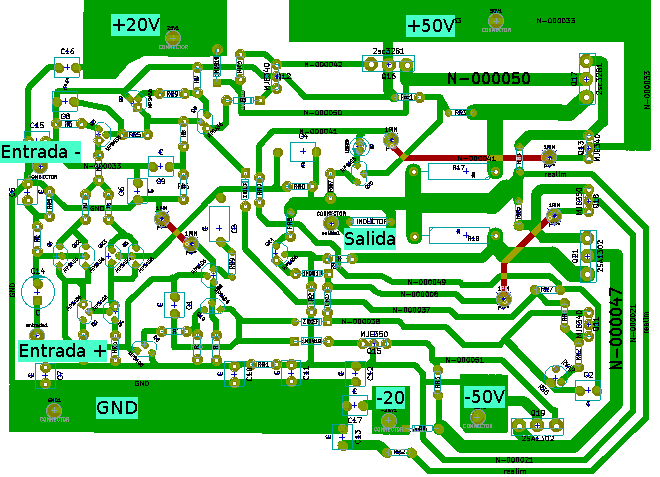
\includegraphics[width=1\textwidth]
{img/PCB1.png}}
\caption{Circuito impreso del amplificador.}
\end{figure}

\subsubsection{Fuente Lineal}
\medskip
Para este circuito se utilizaron pistas de 4mm de ancho. Los diodos utilizados en el puente son 6A10 los cuales pueden soportar las corrientes requeridas por el amplificador, ya que soportan hasta 6A; y poseen una caída de tension en directa menor a 1V.
En la Figura~\ref{circuito_impreso_fuente_lineal} se muestra el circuito impreso implementado. 



\begin{figure}[H]
\centering
\centerline{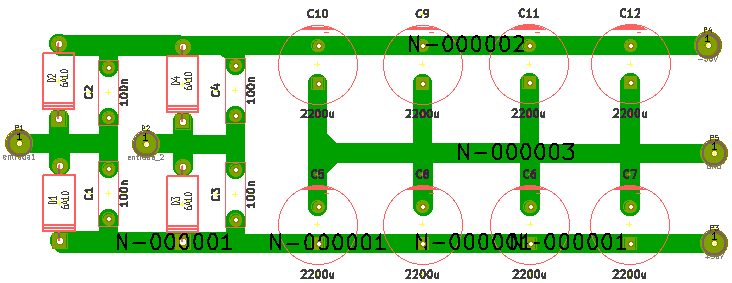
\includegraphics[width=1\textwidth]{img/circuito_impreso_fuente_lineal.png}}
\caption{Circuito impreso de la fuente lineal.}
\label{circuito_impreso_fuente_lineal} 
\end{figure}
\medskip
\subsubsection{Preamplificador}

En este impreso se debió tener en cuenta las posiciones y sentido de giro de los potenciometros para lograr un frente coherente y ordenado. Se agrego un conector jack a la salida para facilitar la desconexión con el amplificador de potencia de ser necesario.
Se utilizaron amplificadores operacionales NE5532, típicos en este tipo de aplicaciones debido a sus buenas prestaciones y bajo ruido.

\begin{figure}[H]
\centering
\centerline{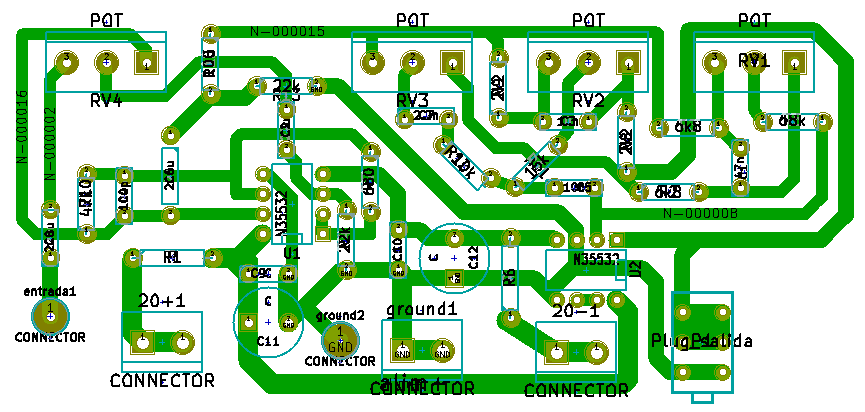
\includegraphics[width=1\textwidth]{img/pre_pcb.png}}
\caption{Circuito impreso del preamplificador.}
\label{pre_pcb} 
\end{figure}

\subsection{Mediciones}

\subsection{Comparativa Mediciones-Simulaciones}
\subsection{Errores y Modificaciones al Diseño Original}

\newpage
\section{Conclusiones}
\newpage
\section{Anexos}

\end{document}

